\begin{figure}[tb]
\centering
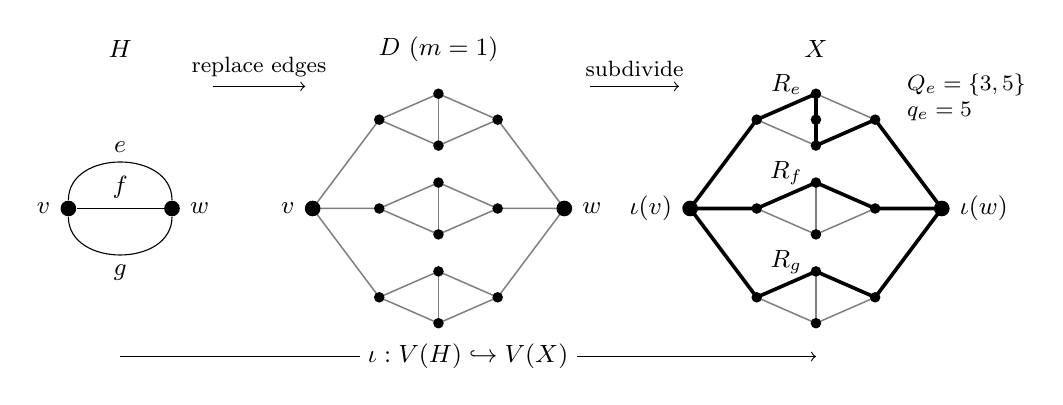
\begin{tikzpicture}[
  x=.94cm,y=.94cm,
  every node/.style={font=\small},
  vertex/.style={circle,fill=black,inner sep=1.35pt},
  branch/.style={circle,fill=black,inner sep=2pt},
  edge/.style={draw=black!50,line width=.55pt},
  chosen/.style={draw=black,line width=1.3pt},
]
\node at (0,2.15) {$H$};
\node at (4.3,2.15) {$D$ ($m=1$)};
\node at (9.4,2.15) {$X$};
\node[branch,label=left:$v$] (hu) at (-.7,0) {};
\node[branch,label=right:$w$] (hv) at (.7,0) {};
\draw (hu) .. controls (-.7,.8) and (.7,.8) .. (hv)
  node[midway,above] {$e$};
\draw (hu)--(hv) node[midway,above] {$f$};
\draw (hu) .. controls (-.7,-.8) and (.7,-.8) .. (hv)
  node[midway,below] {$g$};

\foreach \offset/\name in {4.3/d,9.4/x} {
  \begin{scope}[xshift=\offset*.94cm]
    \coordinate (\name u) at (-1.7,0);
    \coordinate (\name v) at (1.7,0);
    \foreach \height/\j in {1.2/e,0/f,-1.2/g} {
      \coordinate (\name a\j) at (-.8,\height);
      \coordinate (\name b\j) at (.8,\height);
      \coordinate (\name c\j) at (0,\height+.35);
      \coordinate (\name d\j) at (0,\height-.35);
      \draw[edge] (\name u)--(\name a\j)--(\name c\j)--(\name b\j)--(\name v);
      \draw[edge] (\name a\j)--(\name d\j)--(\name b\j);
      \draw[edge] (\name c\j)--(\name d\j);
    }
  \end{scope}
}
\node[branch,label=left:$v$] at (du) {};
\node[branch,label=right:$w$] at (dv) {};
\node[branch,label=left:$\iota(v)$] at (xu) {};
\node[branch,label=right:$\iota(w)$] at (xv) {};
\coordinate (xs) at (9.4,1.2);
\draw[chosen] (xu)--(xae)--(xce)--(xs)--(xde)--(xbe)--(xv);
\draw[chosen] (xu)--(xaf)--(xcf)--(xbf)--(xv);
\draw[chosen] (xu)--(xag)--(xcg)--(xbg)--(xv);
\foreach \name in {d,x} {
  \foreach \j in {e,f,g} {
    \foreach \p in {a,b,c,d} {\node[vertex] at (\name\p\j) {};}
  }
}
\node[vertex] at (xs) {};
\foreach \height/\j in {1.2/e,0/f,-1.2/g} {
  \node at (9,\height+.48) {$R_\j$};
}
\node[align=left,font=\footnotesize,anchor=west] at (10.5,1.5)
  {$Q_e=\{3,5\}$\\$q_e=5$};
\draw[->] (1.25,1.65)--(2.5,1.65)
  node[midway,above,font=\footnotesize] {replace edges};
\draw[->] (6.35,1.65)--(7.55,1.65)
  node[midway,above,font=\footnotesize] {subdivide};
\draw[->] (0,-2)--(9.4,-2)
  node[midway,fill=white,inner sep=3pt] {$\iota:V(H)\hookrightarrow V(X)$};
\end{tikzpicture}
\caption{The construction in \cref{lem:independent-path-lengths}.
Each edge of $H$ is replaced by a diamond in $D$.
In $X$, the vertical edge of the top diamond is subdivided once.
The bold paths form the chosen subdivision of $H$.
The paths for $e$ have four or six edges, so $Q_e$ lists their possible
internal-vertex counts.}
\label{fig:diamond-objects}
\end{figure}
